\documentclass[aspectratio=169]{beamer}

% --- Theme Configuration ---
\usetheme{Berlin} 
\usecolortheme{whale} 

\usepackage{booktabs}
\usepackage{graphicx}
\usepackage{amsmath}

% --- Presentation Metadata ---
\title[DI-Quantum Comm]{Device-Independent Quantum Communication Technology}
\subtitle{From Theory to Hardware Security}
\author{Prince Kumar (230051013)}
\institute{Indian Institute of Technology Indore}
\date{April 23, 2026}

\begin{document}

% --- Title Slide ---
\begin{frame}
    \titlepage
\end{frame}

% --- Slide 2: Agenda ---
\begin{frame}{Agenda}
    \begin{itemize}
        \item \textbf{The Security Gap:} Quantum Promise vs. Physical Reality
        \item \textbf{Theoretical Foundations:} EPR Paradox and Bell's Theorem
        \item \textbf{Hardware Architecture:} Engineering Entanglement
        \item \textbf{Vulnerabilities:} The APD Blinding Exploit
        \item \textbf{The Solution:} Device-Independent QKD (DI-QKD)
        \item \textbf{True Randomness:} QRNGs and Bias Extraction
    \end{itemize}
\end{frame}

% --- Section 1: Introduction ---
\section{The Security Gap}
\begin{frame}{The Quantum Promise vs. Physical Reality}
    \begin{itemize}
        \item \textbf{Information-Theoretic Security:} Guaranteed by No-Cloning and Wave-function Collapse.
        \item \textbf{The Physical Gap:} Ideal proofs ignore fiber loss ($\alpha \approx 0.2$ dB/km) and hardware imperfections.
        \item \textbf{Security Collapse:} If detection hardware is compromised, the mathematical model of the quantum state becomes invalid.
    \end{itemize}
    \begin{block}{Shor-Preskill Threshold}
        Secure key extraction is only possible if the Quantum Bit Error Rate (QBER) remains below $\approx 11\%$.
    \end{block}
\end{frame}

% --- Section 2: Theoretical Foundations ---
\section{Bell's Theorem}

\begin{frame}{Quantum Entanglement}
    \begin{columns}
        \begin{column}{0.5\textwidth}
            \begin{itemize}
                \item \textbf{Definition:} A phenomenon where particles become intrinsically linked, such that the quantum state of one is inseparable from the others.
                \item \textbf{Non-Local Correlation:} Measuring one particle instantaneously determines the state of its entangled partner, regardless of physical distance.
                \item \textbf{Superposition Collapse:} The act of measurement collapses the shared wave-function simultaneously.
                \item \textbf{Foundation of QKD:} Any eavesdropping attempt automatically breaks the entangled state, introducing detectable errors that compromise security.
            \end{itemize}
        \end{column}
        \begin{column}{0.5\textwidth}
            \begin{figure}
                \centering
                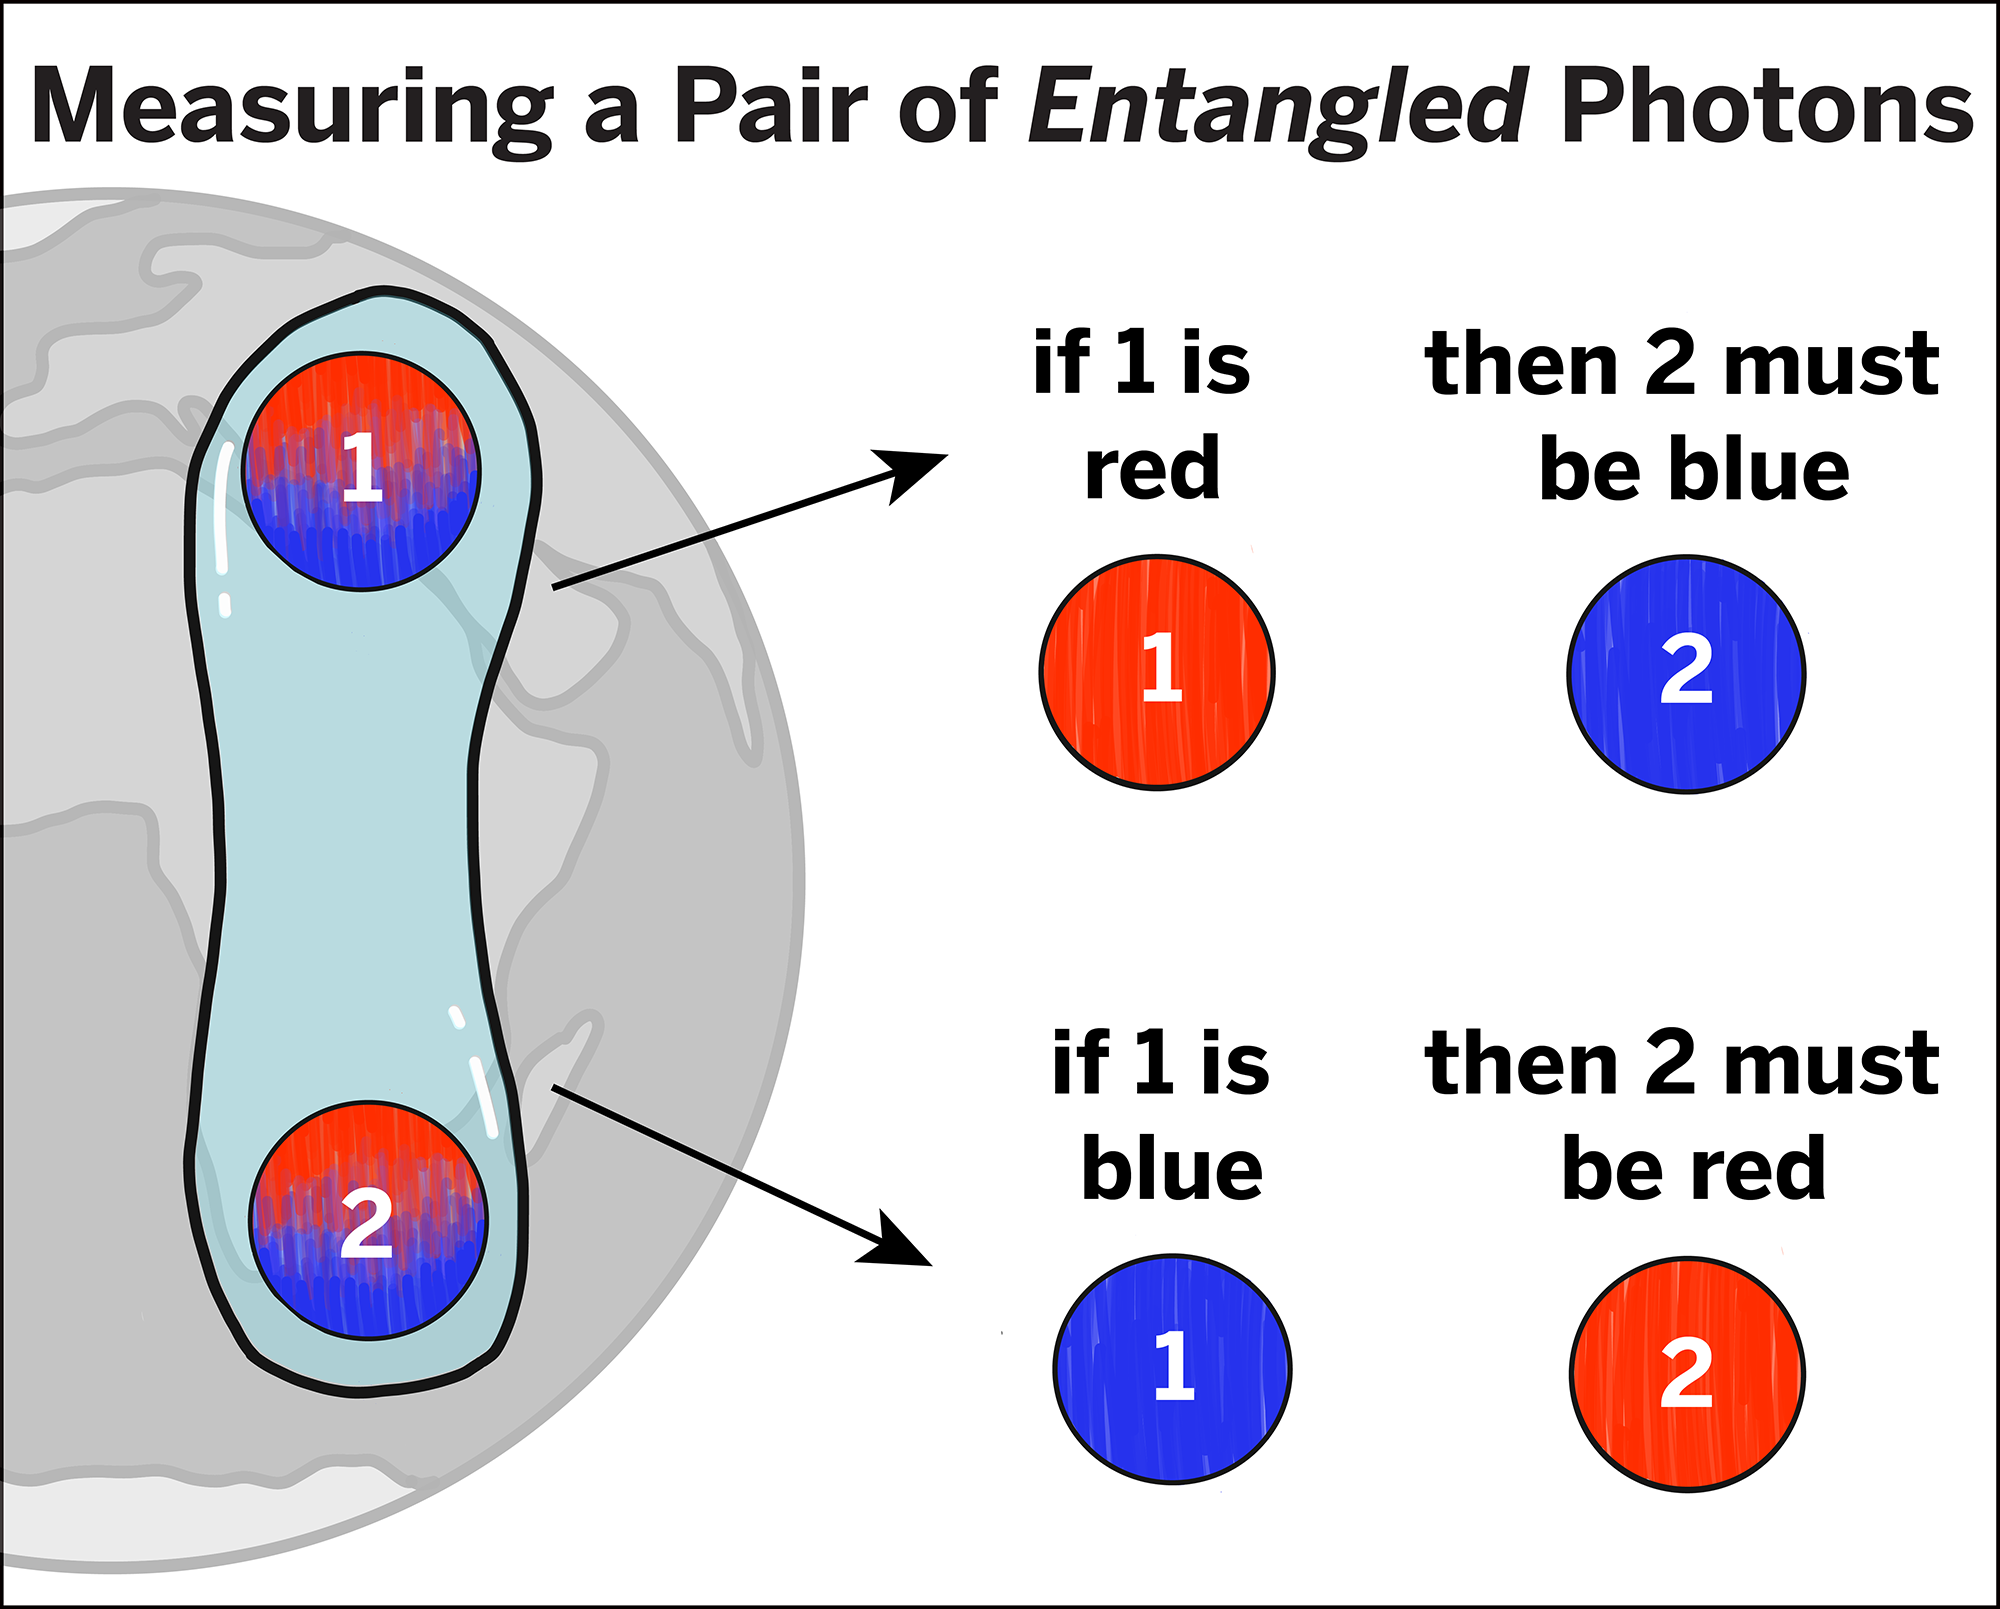
\includegraphics[width=\linewidth]{figures/entanglement_chart.png}
                \caption{Representation of Quantum Entanglement \cite{quantum_atlas}}
            \end{figure}
        \end{column}
    \end{columns}
\end{frame}

\begin{frame}{EPR Paradox and the CHSH Inequality}
    \begin{columns}
        \begin{column}{0.6\textwidth}
            \begin{itemize}
                \item \textbf{Local Realism:} Einstein's argument for "Hidden Variables" to avoid "spooky action".
                \item \textbf{CHSH Inequality (1964):} Tests correlations between Alice and Bob at varying angles.
                \item \textbf{Realism vs. QM:} Violation proves measurement actively defines reality.
            \end{itemize}
            \begin{alertblock}{Mathematical Bounds}
                Classical Hidden Variables: $S \le 2$ \\
                Tsirelson's Bound (Quantum): $S = 2\sqrt{2} \approx 2.828$
            \end{alertblock}
        \end{column}
        \begin{column}{0.4\textwidth}
            \centering
            \textbf{Bell State:} \\
            $|\Phi^{+}\rangle = \frac{1}{\sqrt{2}}(|HH\rangle + |VV\rangle)$ \\
            \vspace{0.5cm}
            \textit{Higher $S$ values indicate stronger non-classical correlation.}
        \end{column}
    \end{columns}
\end{frame}

% --- Section 3: Hardware Engineering ---
\section{Optical Architecture}
\begin{frame}{Engineering Entanglement: The BBM92 Setup}
    \begin{figure}
        \centering
        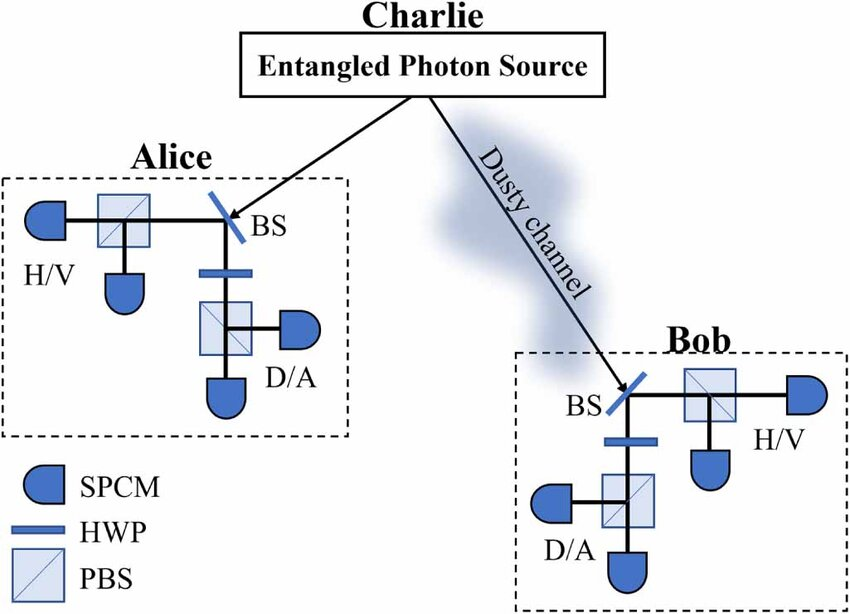
\includegraphics[width=0.6\linewidth]{figures/bbm92 (1).png}
        \caption{BBM92 Architecture: An untrusted central source (Charlie) distributes photons to Alice and Bob \cite{bbm92_diagram}}
    \end{figure}
\end{frame}

\begin{frame}{The 4-Step Engineering Process}
    \begin{columns}
        \begin{column}{0.5\textwidth}
            \begin{enumerate}
                \item \textbf{Generation:} SPDC via non-linear crystals (BBO/ppKTP).
                \item \textbf{Superposition:} Path overlap to erase "which-path" info.
                \item \textbf{Compensation:} Fixing phase errors via $YVO_4$.
                \item \textbf{Splitting:} Wedge mirrors separate signal/idler.
            \end{enumerate}
        \end{column}
        \begin{column}{0.5\textwidth}
            \begin{figure}
                \centering
                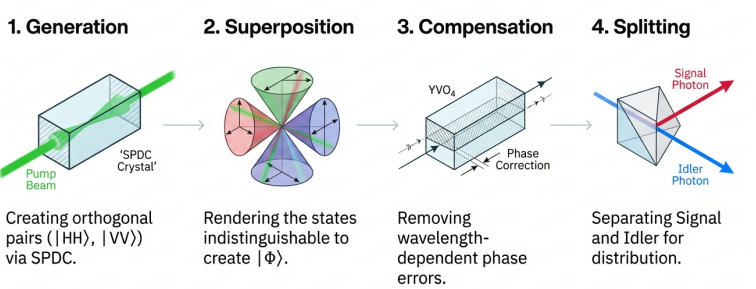
\includegraphics[width=\linewidth]{figures/generation.png}
                \caption{Entanglement Generation Process.}
            \end{figure}
        \end{column}
    \end{columns}
\end{frame}

% --- Section 4: Vulnerabilities ---
\section{Hardware Attacks}
\begin{frame}{The Detector Blinding Exploit (Gerhardt et al.)}
    \begin{figure}
        \centering
        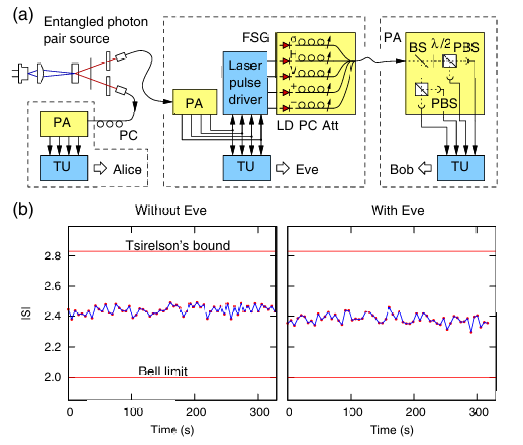
\includegraphics[width=0.65\linewidth]{figures/faking_bell.png}
        \caption{Experimental setup for faking Bell violations using a Faked-State Generator (FSG).}
    \end{figure}
    \begin{alertblock}{The "Hack" Results}
        Eve achieves an unphysical score of $S \approx 2.797$. Alice and Bob remain unaware due to the \textbf{Fair Sampling Assumption}.
    \end{alertblock}
\end{frame}

\begin{frame}{Countermeasures: Defending the Detectors}
    \begin{itemize}
        \item \textbf{High-Energy Laser Detection:} Integrating an optical power meter or dedicated watchdog detector at the receiver's entrance.
        \item \textbf{Continuous Monitoring:} The watchdog continuously profiles incident optical power against the expected single-photon threshold.
        \item \textbf{Abort Protocol:} If power exceeds the threshold, the system flags a blinding laser attack and immediately aborts key distribution.
        \item \textbf{The "Arms Race":} Physical patches often lead to new, creative quantum hacking techniques, underscoring the need for hardware-independent security (DI-QKD).
    \end{itemize}
\end{frame}

% --- Section 5: The DI-QKD Solution ---
\section{DI-QKD}
\begin{frame}{Device-Independent QKD: The Zero-Trust Model}
    \begin{itemize}
        \item \textbf{Black Box Approach:} Treat all hardware as untrusted; security relies on statistical outputs.
        \item \textbf{Verification:} Use the Bell test directly on hardware. $S > 2$ ensures security.
        \item \textbf{Monogamy of Entanglement:} A third party (Eve) cannot correlate with a maximally entangled pair.
    \end{itemize}
    \begin{block}{Paradigm Shift}
        Moves from modeling the \textbf{internal physics} of a device to verifying the \textbf{external correlations}.
    \end{block}
\end{frame}

% --- Section 6: QRNG & Conclusion ---
\section{True Randomness}
\begin{frame}{Closing the Loophole: QRNGs}
    \begin{itemize}
        \item \textbf{Unpredictability:} DI-QKD fails if Eve predicts measurement bases.
        \item \textbf{Quantum Randomness:} Spatial superposition in a 50/50 beam splitter.
        \item \textbf{Von Neumann Extractor:} Eliminates hardware bias by processing non-overlapping bit pairs.
    \end{itemize}
    \begin{exampleblock}{Extractor Logic}
        Input: '01' $\rightarrow$ Output: 0 \\
        Input: '10' $\rightarrow$ Output: 1 \\
        Discard: '00' and '11'
    \end{exampleblock}
\end{frame}

\begin{frame}{Conclusion}
    \begin{itemize}
        \item Physical layer vulnerabilities (APDs) compromise standard QKD.
        \item DI-QKD provides security even when devices are fundamentally compromised.
        \item Future networks must integrate robust Bell tests and bias-extracted QRNGs.
    \end{itemize}
    \vspace{0.5cm}
    \centering
    \LARGE \textbf{Thank You!} \\
    \small \textit{Questions?} \\
    \footnotesize Simulation: \href{https://princekumarofficial.github.io/rng-von-neumann-extractor/}{https://princekumarofficial.github.io/rng-von-neumann-extractor/}
\end{frame}

\begin{frame}
    \frametitle{References}
    \begin{thebibliography}{10}
        \bibitem{quantum_atlas}
        Quantum Atlas, University of Maryland.
        \newblock \href{https://quantumatlas.umd.edu/entry/entanglement/}{Entanglement.}
        
        \bibitem{bbm92_diagram}
        ResearchGate.
        \newblock \href{https://www.researchgate.net/figure/The-block-diagram-of-implemented-BBM92-protocol-HWP-half-wave-plate-PBS-polarizing_fig1_360556529}{BBM92 protocol block diagram.}
    \end{thebibliography}
\end{frame}

\end{document}.